% v0.21: foreground-cut derivation and explicit block-error definition, 2026-10-29.
% Compile with XeLaTeX or Tectonic; source/data TODOs remain for the author.
% Scientific arrays and previous versions are preserved.
\documentclass[fleqn,usenatbib]{mnras}
% MNRAS controls page geometry, body spacing and captions.
\usepackage[T1]{fontenc}
\usepackage{newtxtext,newtxmath}
\usepackage{amsmath,bm}
\usepackage{graphicx,booktabs,longtable,array,calc}
\usepackage[export]{adjustbox}
\usepackage{placeins,float}
\usepackage{xcolor}
\usepackage{bookmark}
\setlength{\emergencystretch}{2em}
\hypersetup{hypertexnames=false,colorlinks=true,linkcolor=blue!40!black,citecolor=blue!40!black,urlcolor=blue!40!black,pdftitle={Redshift evolution of the HI-weighted genus under Alcock-Paczynski distortions and foreground filtering}}
\providecommand{\tightlist}{\setlength{\itemsep}{0pt}\setlength{\parskip}{0pt}}
\newcommand{\pandocbounded}[1]{#1}
\DeclareRobustCommand{\todo}[1]{\textcolor{red!65!black}{\textbf{[TODO: }#1\textbf{]}}}

% Avoid artificial vertical stretching while retained wide figures float.
\raggedbottom
\XeTeXtracingfonts=0

\hypersetup{pdfauthor={Wells}}
\title[Genus evolution, AP and foreground filtering]{Redshift evolution of the H\,I-weighted genus under Alcock--Paczy\'nski distortions and foreground filtering}
\author{}
\date{}
\pubyear{2026}
\begin{document}
\label{firstpage}
\pagerange{\pageref{firstpage}--\pageref{lastpage}}
\maketitle
\begin{abstract}
We investigate how foreground mode removal affects the redshift evolution of the H\,I-weighted genus and its response to Alcock--Paczy\'nski (AP) distortions. Using four Jiutian 1G snapshots at $0.10\le z\le0.59$, we construct H\,I mass-weighted fields and measure their genus at a Gaussian smoothing scale of $20\,h^{-1}\mathrm{Mpc}$ under idealized horizontal and wedge cuts. The horizontal cut raises the fitted genus amplitude by a factor of about 4.6, despite reducing the field variance. In the simulation cosmology, the curves show modest evolution over the sampled redshifts; their endpoint changes do not describe the full intermediate variation. Subtracting this intrinsic evolution leaves redshift-dependent residuals under the tested incorrect distance--redshift relations, showing that the filtered measurement retains a response to the assumed geometry. The resulting parameter regions depend strongly on their numerical construction. Tests identify discontinuities associated with integer mesh changes and sharp Fourier masks, while parameter-space smoothing changes the relative region areas. We therefore interpret these regions as exploratory summaries of the simulated pipeline response, rather than calibrated cosmological precision. The results motivate further tests of H\,I topology with numerically stable measurements and realistic foreground models.

\end{abstract}
\begin{keywords}
large-scale structure of Universe -- cosmology: theory -- methods: numerical -- neutral hydrogen -- topology
\end{keywords}
\section{Introduction}\label{sec:intro}
Within the standard cosmological model, dark energy drives the late-time accelerated expansion, but its physical origin remains uncertain \citep{PeeblesRatra2003DarkEnergy,Li2011DarkEnergy}. Testing whether it is a cosmological constant or evolves with time requires measurements of the expansion history and the growth of structure \citep{Weinberg2013Acceleration}. The large-scale distribution of galaxies provides a way to investigate these questions.

Galaxy clustering constrains distances and structure growth through two-point statistics, baryon acoustic oscillations, redshift-space distortions and the Alcock--Paczy\'nski (AP) effect \citep{Tegmark2004SDSS,BlakeGlazebrook2003BAO,SeoEisenstein2003BAO,Eisenstein2005BAO,Kaiser1987,Ballinger1996AP,Alam2017BOSS}. These applications motivate complementary probes of the geometry and connectivity of large-scale structure \citep{Blake2011Growth,Blake2011AP,Beutler2017Anisotropic}.

The genus characterizes the topology of the large-scale density field, complementing the power spectrum and two-point correlation function \citep{Hamilton1986Topology,Mecke1994,SchmalzingBuchert1997Morphology}. At a fixed smoothing scale, a uniform positive rescaling of the density contrast preserves the genus curve expressed in volume-fraction thresholds \citep{Matsubara2003SmoothedFields,Wang2012TopologyGravity}, motivating its use in studies of redshift evolution. Topological measurements in the 2dF Galaxy Redshift Survey, SDSS luminous red galaxy sample and WiggleZ survey provide observational applications of these statistics \citep{Park2005SDSS,James2009Topology2dF,Gott2009LRGGenus,Blake2014WiggleZTopology}. Simulations also show that genus evolution depends on tracer bias and gravitational growth \citep{Park2005Evolution}. More recently, the four Minkowski functionals of BOSS galaxies have been analysed with a simulation-based model for cosmological inference \citep{Liu2025}.

\citet{ParkKim2010Ruler} proposed using large-scale topology as a cosmic standard ruler, motivating comparisons of the genus across redshifts. This approach was developed through mock-catalogue tests of the genus amplitude \citep{Appleby2018} and measurements of the expansion history from the two-dimensional genus of observed galaxies \citep{Appleby2021GenusExpansion}. These studies provide the main motivation for examining whether H\,I topology retains a useful redshift-dependent geometric response after foreground filtering.

H\,I intensity mapping traces large-scale structure through integrated 21-cm emission \citep{Battye2013IntensityMapping}, and its clustering depends on how H\,I populates dark matter haloes \citep{Villaescusa2018}. Topology has been proposed as a probe of the H\,I distribution with the Square Kilometre Array (SKA) \citep{Wang2015HITopologySKA}. Minkowski functionals have also been used to study the H\,I--halo mass relation in two-dimensional intensity maps with foreground filtering \citep{Spina2021HIHaloMF}.

An assumed cosmology is required to convert redshifts and angles into comoving positions. An incorrect distance--redshift relation introduces redshift-dependent AP distortions, which can alter the measured genus at a fixed smoothing scale \citep{AlcockPaczynski1979}. Following the redshift-differencing approach of tomographic AP analyses \citep{Li2014GradientAP,Li2016TomographicAP,Park2019EvolutionAP}, we compare the full three-dimensional genus curves of H\,I mass-weighted fields across redshifts after subtracting the intrinsic evolution measured in the simulation cosmology.

Foreground avoidance in 21-cm surveys removes contaminated Fourier modes at low line-of-sight wavenumbers and within the foreground wedge \citep{SeoHirata2016Wedge}. The wedge arises from mode mixing in the chromatic interferometer response \citep{Datta2010BrightSourceWedge,Morales2012ForegroundShapes}. We use idealized line-of-sight and wedge cuts to examine how mode removal affects the redshift evolution of the H\,I-weighted genus and its sensitivity to the assumed cosmology. The cuts are not calibrated to a specific instrument. Frequency-dependent beam errors can introduce additional foreground leakage \citep{Ding2024BeamCalibration}; this instrumental effect is not included here.

We address three questions: how foreground removal changes the genus and its evolution in the simulation cosmology; whether redshift-differenced genus measurements retain a response to an incorrect distance--redshift relation; and how reliably the resulting parameter regions can be compared. Sections~\ref{sec:data}--\ref{sec:statistics} describe the samples, measurement and statistic. Section~\ref{sec:results} presents the field morphology, genus evolution, geometric response and parameter regions, together with numerical sensitivity tests. Section~\ref{sec:discussion} discusses their implications for H\,I surveys.

\section{Simulation and samples}\label{sec:data}
The Jiutian simulation suite was developed to support the extragalactic surveys of the China Space Station Telescope (CSST; \citealt{Jiutian2025Overview}). It combines primary runs at different resolutions, the Kun runs sampling cosmological parameters \citep{Chen2025Kun}, extensions with massive neutrinos \citep{Chen2025Neutrinos,Yu2026CUBE2}, warm dark matter \citep{He2023WarmDM} and interacting dark energy \citep{Zhang2019IDE}, and constrained zoom simulations of regions in the observed Universe \citep{Luo2024ELUCID}. The primary runs also provide the basis for mock galaxy catalogues built with semi-analytical models \citep{Pei2024Emission,Tan2026GAEA} and subhalo abundance matching \citep{Gu2024SHAM}, as well as catalogues and synthetic observations for the CSST imaging surveys \citep{Wei2026MockCatalog,Wei2026Framework}.

We use four snapshots from Jiutian 1G, a dark-matter-only $N$-body run in a periodic box of side $1000\,h^{-1}\mathrm{Mpc}$. The published run evolves $6144^3$ particles with a particle mass of $3.723\times10^8\,h^{-1}\mathrm{M}_{\odot}$ and a comoving gravitational softening of $4\,h^{-1}\mathrm{kpc}$ \citep{Jiutian2025Overview}. Its flat $\Lambda$CDM cosmology has $\Omega_{m,\mathrm{sim}}=0.3111$, $\Omega_b=0.049$, $h=0.6766$, $n_s=0.9665$, $\sigma_8=0.8102$ and $w_{\mathrm{sim}}=-1$. The snapshots span $z=0.10$--$0.59$; their redshifts and selected sample sizes are listed in Table~\ref{tab:snapshots}. \todo{Confirm the H\,I assignment model and the provenance of the specific galaxy catalogue used here.}

\begin{table}
\centering
\caption{Snapshots and sample sizes.}
\label{tab:snapshots}
\begin{tabular}{@{}lrr@{}}
\toprule
Snapshot & Redshift & Objects \\
\midrule
118 & 0.10235 & $10^6$ \\
112 & 0.19095 & $10^6$ \\
105 & 0.31970 & $10^6$ \\
94 & 0.59339 & $10^6$ \\
\bottomrule
\end{tabular}
\end{table}

At each snapshot, we retain objects with finite positions, velocities and positive finite H\,I masses, select the $10^6$ objects with the largest H\,I masses, and weight them by H\,I mass. Selection is performed independently at each redshift. We also analyse all valid objects with positive H\,I mass as a sample-selection comparison.

\section{Measurement}\label{sec:measurement}
\subsection{Redshift-space distortions and AP mapping}
Peculiar velocities can change the genus amplitude even in linear theory \citep{Matsubara1996IsodensityRedshift}. We adopt the plane-parallel approximation with the $z$-axis as the line of sight. To first order in $v_\parallel/c$ \citep{DavisScrimgeour2014Peculiar}, the redshift-space position in the simulation cosmology is
\begin{equation}
s_\parallel=x_\parallel+\frac{(1+z)v_\parallel}{100E(z;\theta_{\mathrm{sim}})},
\end{equation}
where $x_\parallel$ is the comoving position in $h^{-1}\mathrm{Mpc}$, $v_\parallel$ is the peculiar velocity in $\mathrm{km\,s^{-1}}$, and $E=H/H_0$. For the flat, constant-$w$ model used here,
\begin{equation}
E^2(z;\theta)=\Omega_m(1+z)^3+(1-\Omega_m)(1+z)^{3(1+w)}.
\end{equation}

We then apply the AP mapping to the redshift-space positions and box lengths for each scan cosmology $\theta=(\Omega_m,w)$, keeping $h$ fixed \citep{Zunckel2011TopologyDE}:
\begin{equation}
\begin{aligned}
s_\perp^{\mathrm{scan}}&=\alpha_\perp s_\perp^{\mathrm{sim}},\\
s_\parallel^{\mathrm{scan}}&=\alpha_\parallel s_\parallel^{\mathrm{sim}},
\end{aligned}
\end{equation}
\begin{equation}
\begin{aligned}
\alpha_\perp&=\frac{D_M(z;\theta)}{D_M(z;\theta_{\mathrm{sim}})},\\
\alpha_\parallel&=\frac{E(z;\theta_{\mathrm{sim}})}{E(z;\theta)}.
\end{aligned}
\end{equation}
Here $D_M$ is the transverse comoving distance \citep{Hogg1999Distances}. The scaling factors are evaluated at the redshift of each snapshot and applied uniformly within that snapshot. Objects displaced beyond a box face are returned through the opposite face after AP rescaling. The subsequent CIC deposition and genus measurement use open boundaries.

\subsection{Density field and foreground cuts}
We construct the H\,I mass-weighted density field using cloud-in-cell (CIC) interpolation. We fix the target cell size at $\Delta_0=4\,h^{-1}\mathrm{Mpc}$ with $n_i\simeq L_i/\Delta_0$ for the AP-rescaled box lengths $L_i$. We conserve deposited mass at the open box boundary and Fourier transform a zero-extended density contrast (Appendix~\ref{app:implementation}). We correct for the CIC window \citep{Jing2005} and apply Gaussian smoothing with $R=20\,h^{-1}\mathrm{Mpc}$ in scan coordinates.

The cosmological 21-cm signal is much fainter than Galactic and extragalactic radio foregrounds. Their relatively smooth frequency spectra concentrate contamination at low $|k_\parallel|$, corresponding to slowly varying structure along the line of sight. A chromatic instrumental response mixes angular and frequency structure, extending contamination into a wedge at low $|k_\parallel|$ and increasing $k_\perp$ \citep{Datta2010BrightSourceWedge,Morales2012ForegroundShapes,SeoHirata2016Wedge}. Foreground avoidance therefore removes cosmological modes together with the contaminated modes.

To isolate the effect of this anisotropic mode loss, we consider three treatments: no foreground cut (noFG), a horizontal cut removing $|k_\parallel|<0.1\,h\,\mathrm{Mpc}^{-1}$, and the horizontal cut combined with a wedge removing $|k_\parallel|\le m k_\perp$. These masks represent the two characteristic geometries of foreground loss: removal of low line-of-sight modes and the additional angular--frequency mixing of an interferometer. They are controlled, idealized treatments, rather than transfer functions calibrated for a particular survey. Both cuts are defined in scan coordinates, with $k_\parallel=k_z$ and $k_\perp=(k_x^2+k_y^2)^{1/2}$. We keep their parameters fixed across redshifts and scan cosmologies and consider eleven slopes spanning $0.294\le m\le1.692$ (Section~\ref{sec:wedgeareas}). We inverse Fourier transform the filtered field and retain the original box region.

The radial cut can be related to a spectral scale through the local frequency--distance conversion. With $\nu_{\rm obs}=\nu_{21}/(1+z)$ and $\mathrm{d}\chi/\mathrm{d}z=c/H(z)$, its absolute Jacobian is
\begin{equation}\label{eq:frequency_distance}
Y(z)\equiv\left|\frac{\mathrm{d}\chi}{\mathrm{d}\nu_{\rm obs}}\right|
=\frac{c(1+z)^2}{H(z)\nu_{21}}.
\end{equation}
For a spectral mode $\exp(2\pi i\eta\nu_{\rm obs})$, $|k_\parallel|=2\pi|\eta|/Y$. An idealized loss of modes with $|\eta|<\eta_{\rm cut}$ therefore corresponds to
\begin{equation}\label{eq:kcut_frequency}
k_{\rm cut}(z)=\frac{2\pi\eta_{\rm cut}}{Y(z)}
=\frac{2\pi H(z)\nu_{21}}{c(1+z)^2\Delta\nu_{\rm cut}},
\end{equation}
where $\Delta\nu_{\rm cut}=\eta_{\rm cut}^{-1}$ is a spectral period, not a channel width \citep{SeoHirata2016Wedge}. These expressions give wavenumbers in $\mathrm{Mpc}^{-1}$ when $Y$ is in $\mathrm{Mpc}\,\mathrm{MHz}^{-1}$ and frequencies are in MHz; the numerical value in $h\,\mathrm{Mpc}^{-1}$ is obtained by dividing by $h$. A cleaning or instrumental model is needed to specify $\eta_{\rm cut}$. Our fixed $0.1\,h\,\mathrm{Mpc}^{-1}$ is an adopted mode-loss threshold, not a value uniquely derived from the snapshots or $R$. Further scale and wedge relations are given in Appendix~\ref{app:kcut}.

Fig.~\ref{fig:foregroundmask} illustrates the retained and removed modes for the cases used in the field and genus comparisons. Increasing $m$ removes more modes at fixed $k_\perp$, but the wedge adds to the horizontal cut only where $m k_\perp>0.1\,h\,\mathrm{Mpc}^{-1}$. The overlaid Gaussian transfer contours show why the effect of this extra removal also depends on the smoothing scale: modes far from the origin are already strongly attenuated.

\begin{figure*}
\centering
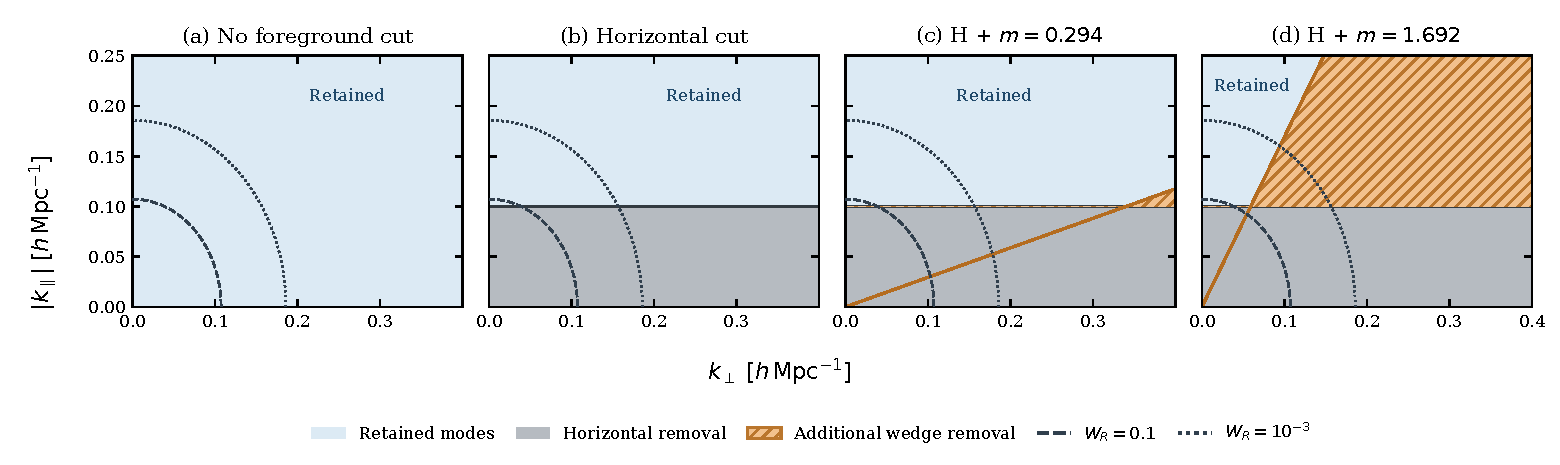
\includegraphics[width=\textwidth]{figures/fig__foreground_kspace.pdf}
\caption{Foreground masks in scan-coordinate Fourier space. Blue marks retained modes, grey the horizontal removal $|k_\parallel|<0.1\,h\,\mathrm{Mpc}^{-1}$, and orange hatching the additional wedge removal. Only $|k_\parallel|\ge0$ is shown; the masks are symmetric in $k_\parallel$. Dashed and dotted arcs indicate the field-amplitude transfer $W_R(k)=\exp[-k^2R^2/2]$ at 0.1 and $10^{-3}$, respectively, for $R=20\,h^{-1}\mathrm{Mpc}$. The diagram shows analytic mask geometry, not a measured power spectrum.}\label{fig:foregroundmask}
\end{figure*}

\subsection{Genus}
The genus describes the connectivity of isodensity surfaces: it distinguishes a network rich in tunnels from isolated high-density regions or enclosed low-density cavities \citep{Hamilton1986Topology,Park2005SDSS}. For the excursion set $E=\{\boldsymbol{x}:\delta(\boldsymbol{x})>\delta_t\}$, we use the cosmological convention $g=-\chi(E)/V$, where $\chi$ is its Euler characteristic and $V$ is the sample volume. Positive genus indicates an excess of tunnels over disconnected components and cavities. We label the density threshold $\delta_t$ by the volume-fraction variable $\nu_f$, defined through
\begin{equation}\label{eq:volumefraction}
f_V(>\delta_t)=\frac{1}{\sqrt{2\pi}}\int_{\nu_f}^{\infty}e^{-u^2/2}\,\mathrm{d}u.
\end{equation}
Thus $\nu_f=0$ selects the upper half of the field volume; it is a Gaussian-equivalent rank threshold, not generally $\delta_t/\sigma$. Comparing fields at fixed $\nu_f$ removes changes caused solely by a uniform positive rescaling of the density contrast \citep{Matsubara2003SmoothedFields}.

In this work, we use 41 equally spaced values over $-2.5\le\nu_f\le2.5$ and determine the corresponding density thresholds separately for each field. We obtain the Euler characteristic from alternating grid-element counts \citep{SchmalzingBuchert1997Morphology}:
\begin{equation}
g(\nu_f)=-\frac{\chi(\nu_f)}{V},\qquad \chi=N_0-N_1+N_2-N_3.
\end{equation}
Here $N_0$, $N_1$, $N_2$ and $N_3$ count vertices, edges, faces and cubes of the excursion set. We use open boundaries, normalize by $V=L_xL_yL_z$ and apply no boundary correction; the counting convention is specified in Appendix~\ref{app:implementation}.

To summarize the amplitude evolution, we fit the Gaussian genus template \citep{Matsubara2003SmoothedFields,Wang2012TopologyGravity}
\begin{equation}
g_{\mathrm{fit}}(\nu_f)=A(1-\nu_f^2)e^{-\nu_f^2/2}
\end{equation}
to the measured curve by equal-weight least squares over $-2.5\le\nu_f\le2.5$. We report the dimensionless amplitude $AR^3$, where $R$ is the Gaussian smoothing scale.

\section{Statistic}\label{sec:statistics}
Following the use of redshift differences and simulation-based evolution corrections in tomographic AP analyses \citep{Li2015Tomographic2PCF,Li2016TomographicAP}, we define an analogous residual for the genus. For each foreground treatment, we take the lowest redshift $z_1$ as the reference and define the intrinsic evolution from the simulation cosmology:
\begin{equation}
\boldsymbol I_i=\boldsymbol g_i(\theta_{\mathrm{sim}})-\boldsymbol g_1(\theta_{\mathrm{sim}}),\qquad i=2,3,4.
\end{equation}
For each scan cosmology $\theta$, we subtract this template from the corresponding redshift difference:
\begin{equation}
\boldsymbol p_i(\theta)=\boldsymbol g_i(\theta)-\boldsymbol g_1(\theta)-\boldsymbol I_i.
\end{equation}
Here $\boldsymbol I_i$ is the intrinsic redshift evolution of the selected, filtered tracer field in the simulation cosmology. Because the same measurements define the template and the residual, $\boldsymbol p_i(\theta_{\mathrm{sim}})=\boldsymbol0$ exactly by construction. An incorrect distance--redshift relation changes the AP scaling with redshift and hence the physical scales selected by fixed scan-coordinate smoothing and foreground cuts; the residual generally no longer vanishes. This is the redshift-dependent response that the statistic tests, not a new simulation of structure growth in each trial cosmology. Fig.~\ref{fig:evolution} shows the non-zero residuals for two illustrative scan cosmologies; the complete curves, including the simulation cosmology, are retained in the supplementary figures. All differences are evaluated at the same 41 volume-fraction thresholds, with a separate template for each foreground treatment.

We concatenate the three residual vectors into a 123-component vector $\boldsymbol p$ and define
\begin{equation}
\chi^2_{\mathrm{int}}(\theta)=\boldsymbol p^{\mathsf T}C^{-1}\boldsymbol p,
\end{equation}
where $C$ includes correlations between thresholds and redshift pairs. This statistic vanishes at the simulation cosmology by construction. For comparison, we also compute the unsubtracted statistic $\chi^2$ using the same covariance. Template subtraction does not necessarily lower the statistic at other cosmologies.

For each foreground treatment, we estimate the covariance at the simulation cosmology using $B=64$ spatial blocks. Let $\boldsymbol t_{ib}$ be block $b$'s additive contribution to the full-volume genus density at redshift $i$, and $f_{ib}$ its grid-volume fraction. The leave-one-out vector is
\begin{equation}\label{eq:jk_loo}
\boldsymbol g_i^{(-b)}=\frac{\boldsymbol g_i-\boldsymbol t_{ib}}{1-f_{ib}}.
\end{equation}
The filtered field and thresholds remain fixed. We concatenate the three paired differences $\boldsymbol g_i^{(-b)}-\boldsymbol g_1^{(-b)}$ into $\boldsymbol d^{(-b)}$ and use
\begin{equation}\label{eq:jk_cov}
C^{\rm JK}_{ab}=\frac{B-1}{B}\sum_{b'=1}^{B}
(d_a^{(-b')}-\bar d_a)(d_b^{(-b')}-\bar d_b),
\end{equation}
where $\bar{\boldsymbol d}=B^{-1}\sum_{b'}\boldsymbol d^{(-b')}$. This retains correlations between thresholds and redshift pairs. The prefactor is the usual equal-block jackknife factor \citep{Norberg2009Errors}; in the implementation it is retained despite small differences in block volume, while Eq.~(\ref{eq:jk_loo}) uses each block's actual fraction. This approximation and the fixed-field interpretation are detailed in Appendix~\ref{app:jackknife}.

The $123\times123$ matrix has rank at most 63. We standardize the centred replicate vectors, apply oracle-approximating shrinkage (OAS; \citealt{Chen2010OAS}) using the scikit-learn implementation \citep{Pedregosa2011ScikitLearn}, and restore the original variances. Equivalently, up to floating-point roundoff,
\begin{equation}\label{eq:jk_oas}
C=(1-\lambda)C^{\rm JK}+\lambda\,\mathrm{diag}(C^{\rm JK}),
\end{equation}
where $\lambda$ is the fitted OAS shrinkage coefficient on the standardized vectors. The regularized covariance is held fixed across scan cosmologies. Curve and paired-difference error bars use $\sqrt{C^{\rm JK}_{aa}}$ from their corresponding replicates; the fixed-covariance residual display uses the matched diagonal of $C$.

We evaluate $\chi^2_{\mathrm{int}}$ at 1285 points in the $(\Omega_m,w)$ plane, concentrated along the degeneracy direction with nominal sampling steps of $\Delta\Omega_m=0.00275$ and $\Delta w=0.01$. We linearly interpolate the weights $\exp(-\chi^2_{\mathrm{int}}/2)$ between sampled points, then smooth the weight surface with a Gaussian kernel of widths $(\sigma_{\Omega_m},\sigma_w)=(0.0069,0.0196)$. These widths follow an empirical rule based on 2.5 times the median nearest-neighbour spacing after scaling the scan rectangle to unit sides. The smoothing reduces variation on the scale of the parameter sampling; its bandwidth has not been independently calibrated as an uncertainty model.

We normalize the smoothed weight within the convex hull of the sampled points and construct highest-density regions containing 68.3, 95.4 and 99.7 per cent of this weight \citep{Hyndman1996HDR}. All parameter contours and area comparisons below use this same construction, including the horizontal-cut reference and the individual redshift pairs. Appendix~\ref{app:area} describes the finite-domain normalization and area evaluation. These regions summarize the conditional parameter response of the simulated analysis; their weight fractions are not independently calibrated confidence levels.

\section{Results}\label{sec:results}
\subsection{Filtered density fields}
Fig.~\ref{fig:slices} compares line-of-sight and transverse slices of the smoothed density field. The noFG field contains interconnected overdense structures and extended underdense regions. After the horizontal cut, the line-of-sight slices develop bands extending in the transverse ($x$ or $y$) direction, with more rapid alternation along the line of sight. Removing low $|k_\parallel|$ suppresses slowly varying radial structure; Gaussian smoothing then favours the surviving modes with relatively small $k_\perp$, producing this transverse coherence. These bands are an imprint of the filter, not additional matter sheets formed by gravitational evolution.

At both displayed redshifts, the horizontal cut reduces the three-dimensional standard deviation from about 0.26 to 0.012. Each panel is normalized by its own field standard deviation, so its colour contrast does not represent the absolute fluctuation amplitude. The $m=0.294$ field remains visually close to the horizontal-cut field, whereas the stronger wedge alters the transverse pattern and further reduces the variance. This follows the mask geometry in Fig.~\ref{fig:foregroundmask}: the weak wedge first adds removal at $k_\perp>0.1/0.294\simeq0.34\,h\,\mathrm{Mpc}^{-1}$, where $R=20\,h^{-1}\mathrm{Mpc}$ smoothing is already severe.

\begin{figure*}
\centering
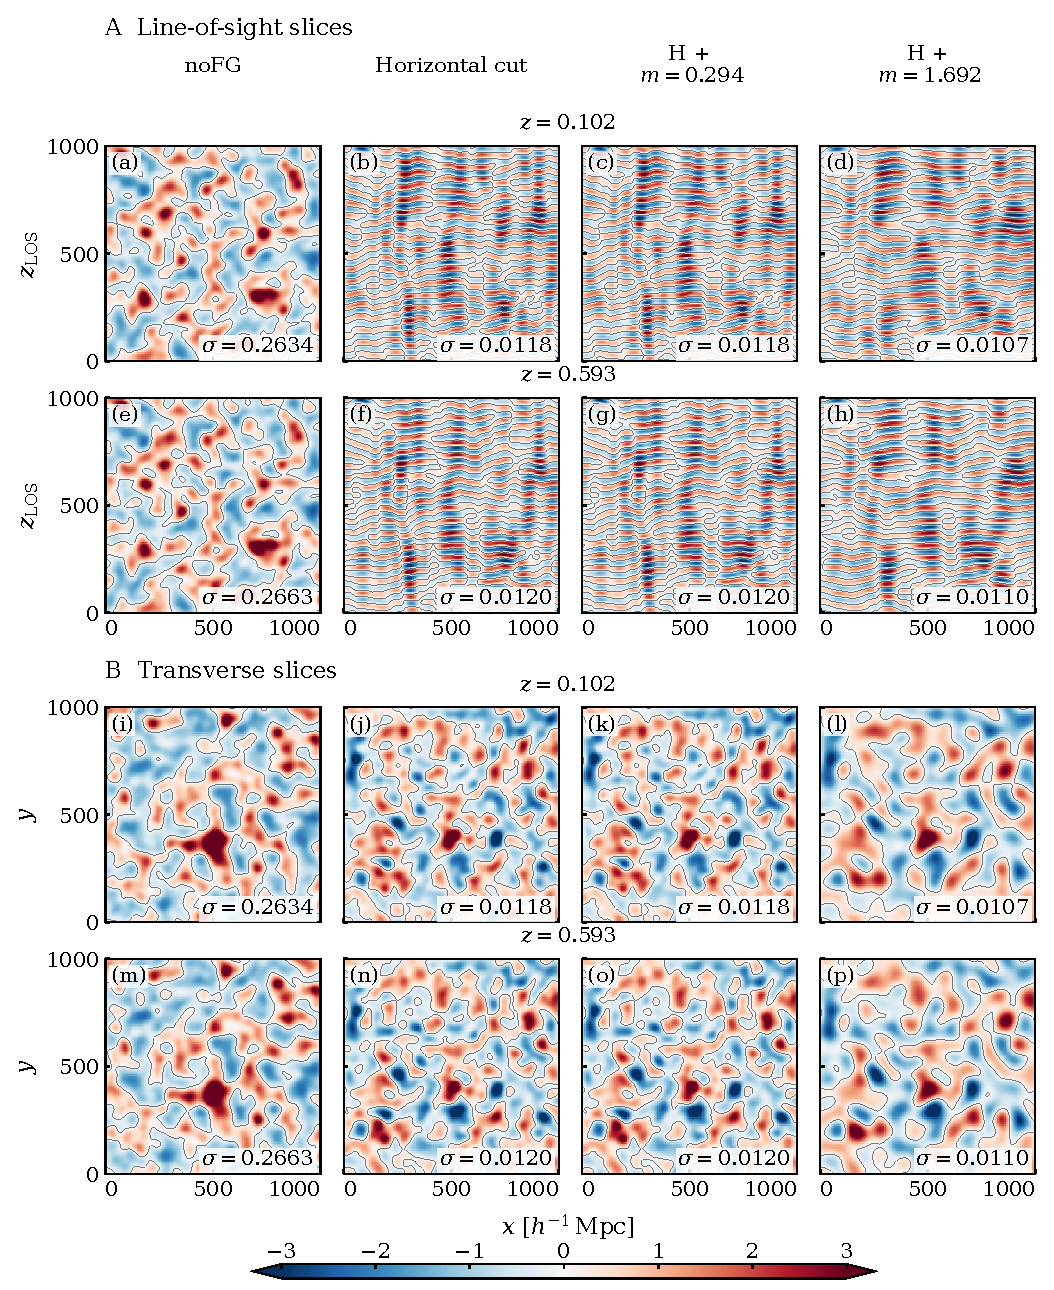
\includegraphics[width=.98\textwidth]{figures/fig__slices.pdf}
\caption{Smoothed H\,I density field in the simulation cosmology at $z=0.102$ and 0.593, normalized by its standard deviation $\sigma_{\rm 3D}$ (labelled $\sigma$ in each panel). A: line-of-sight slices at $y=498\,h^{-1}\mathrm{Mpc}$; B: transverse slices at $z_{\rm LOS}=498\,h^{-1}\mathrm{Mpc}$. Contours mark the median of each three-dimensional field; the colour scale is $\delta_{\rm filtered}/\sigma_{\rm 3D}$, clipped at $\pm3$. All spatial coordinates are in $h^{-1}\mathrm{Mpc}$.}\label{fig:slices}
\end{figure*}

\subsection{Genus curves and intrinsic evolution}
Fig.~\ref{fig:foregroundcurves} shows how foreground removal changes the genus curve at $z=0.102$. The horizontal cut raises the fitted amplitude by about a factor of 4.6, while the strong wedge reduces it relative to the horizontal-cut case. The lower field variance in Fig.~\ref{fig:slices} does not imply a lower genus amplitude: at fixed volume fraction, genus measures connectivity rather than the absolute density contrast. Selective mode removal changes characteristic spatial scales and directional coherence, so it can change the number of tunnels and disconnected regions per unit volume even while suppressing fluctuations. In Gaussian-field theory the amplitude depends on normalized field gradients and their anisotropy \citep{Matsubara1996IsodensityRedshift}; this provides a qualitative interpretation, not a prediction of the measured factor of 4.6.

The weakest wedge ($m\simeq0.294$) matches the displayed horizontal-cut curve because the additional removed modes are strongly suppressed by Gaussian smoothing (Fig.~\ref{fig:foregroundmask}). A stronger wedge reaches modes that survive the smoothing and changes the transverse coherence, consistent with the lower amplitude in Fig.~\ref{fig:foregroundcurves}. The horizontal-cut and weakest-wedge joint statistics agree at 1284 of the 1285 scan points.

\begin{figure}
\centering
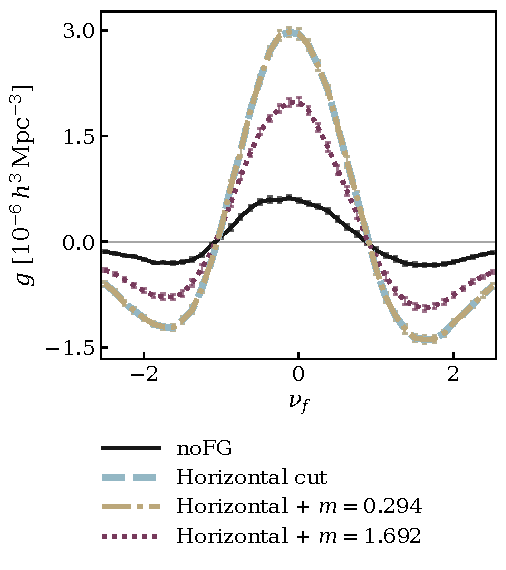
\includegraphics[width=\columnwidth]{figures/fig__noFG_hcut_msan_comp.pdf}
\caption{Genus curves at $z=0.102$ in the simulation cosmology for the four foreground treatments. Error bars are from the 64-block fixed-field jackknife estimate.}\label{fig:foregroundcurves}
\end{figure}

Fig.~\ref{fig:redshifts} separates the nearly overlapping genus curves in its upper row from their small redshift differences below. In the simulation cosmology, the curves change little between $z=0.10$ and 0.59, but the lower panels retain the threshold dependence needed to define $\boldsymbol I_i$. A common growth of the density amplitude alone would cancel at fixed volume fraction; the remaining evolution can reflect nonlinear growth, tracer selection and redshift-space effects, whose individual contributions are not separated here. Table~\ref{tab:amplitudes} lists all three higher-redshift changes relative to $z_1=0.10235$, separately for each sample and foreground treatment. Without foreground cuts, the endpoint fitted amplitude changes by $+0.11$ per cent for the top-$10^6$ sample and $+2.9$ per cent for the full valid catalogue. These changes are descriptive, not significance estimates: their uncertainties require cross-redshift covariance. For the horizontal-cut top-$10^6$ sample, the intermediate snapshots differ from the lowest-redshift amplitude by $-1.44$ and $-1.40$ per cent, although the endpoint difference is only $+0.25$ per cent. Thus a small endpoint change does not imply negligible evolution throughout the interval. The analysis below uses the full curves rather than the fitted amplitudes.

\begin{table*}
\centering
\caption{Redshift evolution of the fitted genus amplitude in the simulation cosmology. Entries give $100[A(z)/A(z_1)-1]$ in per cent, with $z_1=0.10235$ as the reference for each sample and foreground treatment. The reference change is zero by definition. Values are rounded to two decimal places; they are descriptive changes, not significance estimates.}
\label{tab:amplitudes}
\begin{tabular}{@{}lrrrrrr@{}}
\toprule
& \multicolumn{3}{c}{Top $10^6$} & \multicolumn{3}{c}{All valid objects} \\
\cmidrule(lr){2-4}\cmidrule(l){5-7}
Filter & $z=0.19095$ & $z=0.31970$ & $z=0.59339$ & $z=0.19095$ & $z=0.31970$ & $z=0.59339$ \\
\midrule
noFG & $+0.01$ & $-0.25$ & $+0.11$ & $+0.45$ & $+1.18$ & $+2.91$ \\
Horizontal cut & $-1.44$ & $-1.40$ & $+0.25$ & $-0.20$ & $-0.30$ & $-0.48$ \\
Horizontal + $m=0.294$ & $-1.44$ & $-1.40$ & $+0.25$ & $-0.20$ & $-0.30$ & $-0.48$ \\
Horizontal + $m=1.692$ & $-1.31$ & $-1.54$ & $+0.22$ & $0.00$ & $+0.17$ & $+0.10$ \\
\bottomrule
\end{tabular}
\end{table*}



\subsection{Cosmological Dependence}
Fig.~\ref{fig:cosmologies} compares the genus at $z=0.593$ under the simulation cosmology and two illustrative distance--redshift relations. The lower panels reveal differences that are less apparent in the overlapping curves above. With smoothing and foreground cuts fixed in scan coordinates, an AP remapping changes their physical scale and direction dependence, as well as the volume used to report genus density. The resulting differences therefore describe the response of this measurement procedure to the assumed cosmology.

Fig.~\ref{fig:covariance} shows how the redshift-difference measurements are weighted. Its diagonal blocks describe correlations between thresholds within a redshift pair, and its off-diagonal blocks describe correlations between pairs that share the same reference snapshot. The patterns change with foreground treatment, so the significance assigned to a residual depends on its shape relative to the covariance, not only on its visible amplitude.

Fig.~\ref{fig:evolution} connects the genus curves to the redshift-difference statistic. The two displayed scan cosmologies retain redshift-dependent residuals after template subtraction; the simulation-cosmology residual is identically zero and is shown with the full curves in Supplementary Fig.~S1. These examples demonstrate a response of the measurement pipeline to the assumed mapping, without separating its physical and numerical contributions. In the simulation cosmology, the unsubtracted joint statistic is $\chi^2=103$--126 across the four treatments. For the two illustrative scan cosmologies, $\chi^2_{\rm int}$ is approximately 290--585 with foreground cuts and 93--124 without them. Intrinsic subtraction need not lower the statistic away from the simulation cosmology. The dimension of the residual vector alone does not give a calibrated significance for these quadratic forms.

\begin{figure*}
\centering
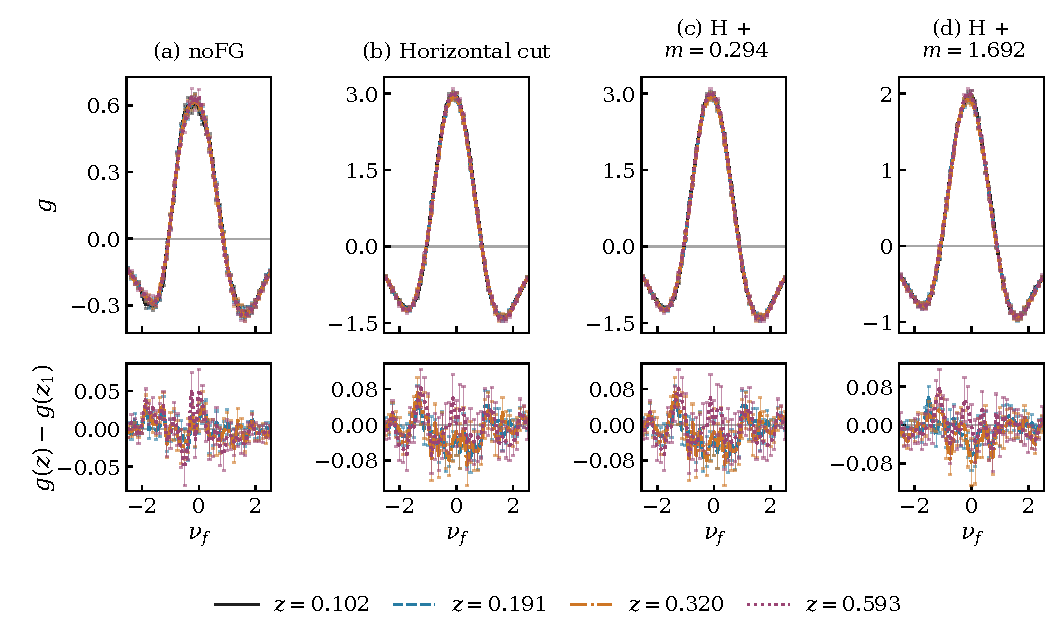
\includegraphics[width=.99\textwidth]{figures/fig__diff_redshifts.pdf}
\caption{Genus curves at the four redshifts in the simulation cosmology (top) and their differences from $z_1=0.102$ (bottom), in units of $10^{-6}h^3\mathrm{Mpc}^{-3}$.}\label{fig:redshifts}

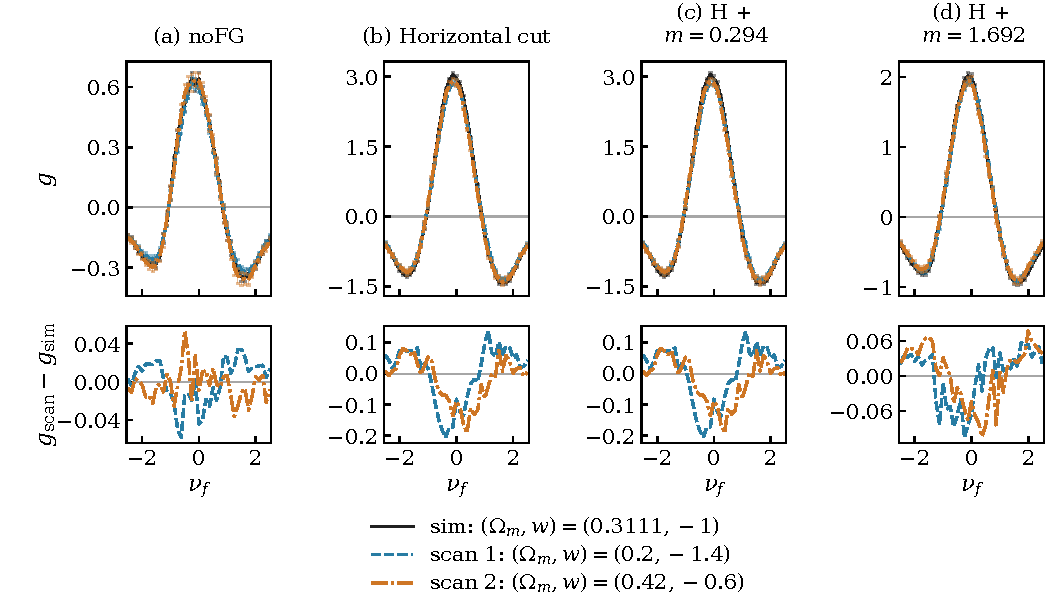
\includegraphics[width=\textwidth]{figures/fig__diff_cosmo.pdf}
\caption{Genus curves at $z=0.593$ in the simulation cosmology and two illustrative cosmologies, $(\Omega_m,w)=(0.2,-1.4)$ and $(0.42,-0.6)$ (top), and their differences from the simulation cosmology (bottom). Values are in units of $10^{-6}h^3\mathrm{Mpc}^{-3}$. The two illustrative points lie outside the 1285-point scan set.}\label{fig:cosmologies}
\end{figure*}

\begin{figure*}
\centering
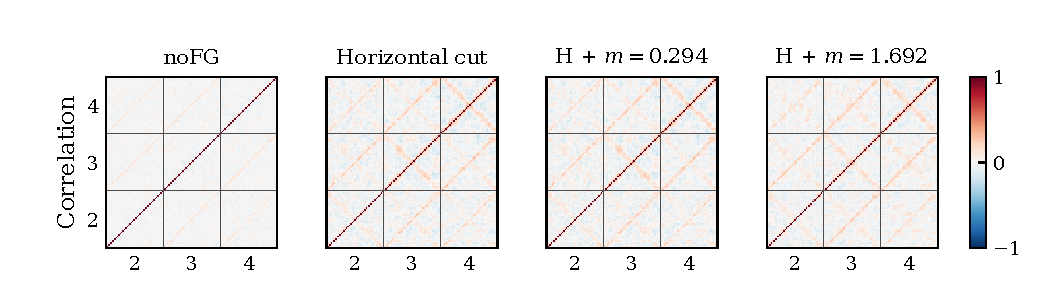
\includegraphics[width=\textwidth]{figures/fig__covmat__correlation.pdf}
\caption{Correlation matrices derived from the regularized covariance of the 123-component difference vector for the four foreground treatments. Axis numbers 2, 3 and 4 identify the redshift pairs $z_i-z_1$, with $\nu_f$ increasing from $-2.5$ to 2.5 within each block. Supplementary Fig.~S4 also shows the covariance amplitudes.}\label{fig:covariance}
\vspace{6pt}
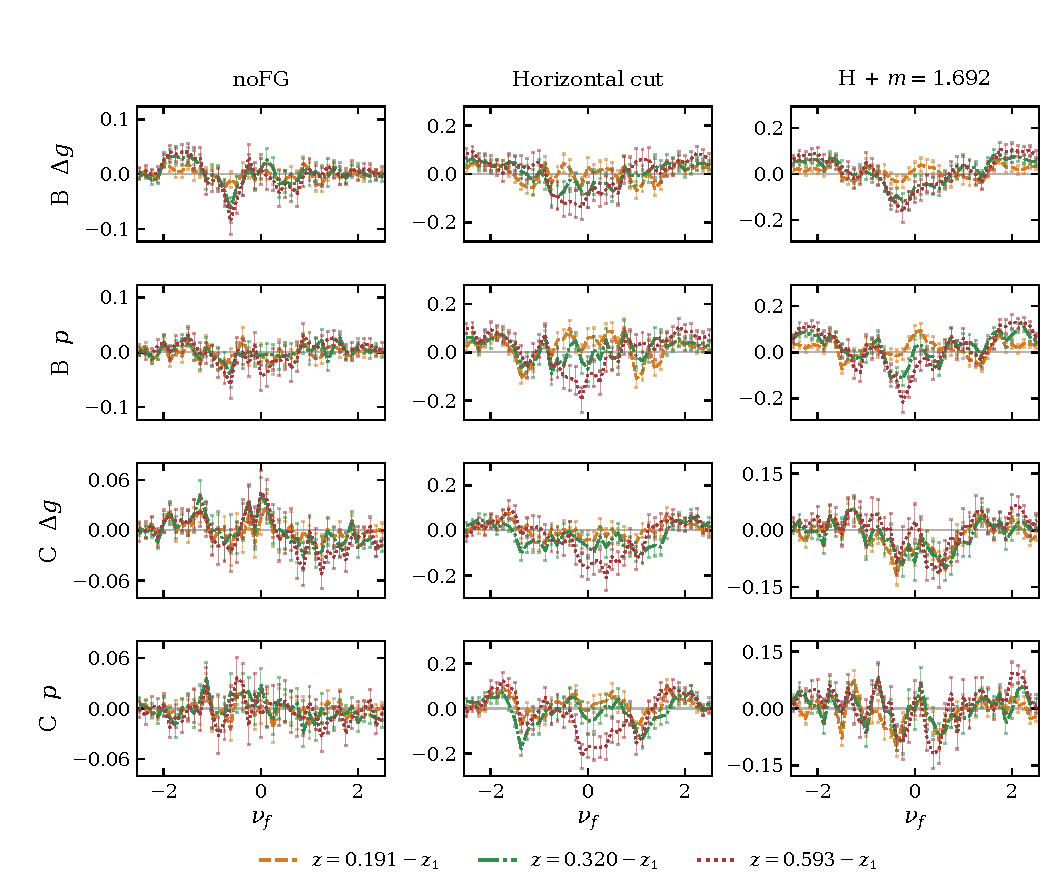
\includegraphics[width=.99\textwidth]{figures/fig__cosmo_redshift_evolution__compact.pdf}
\caption{Redshift differences $\Delta g=g(z_i)-g(z_1)$ and intrinsic-subtracted residuals $p=\Delta g-I$ for two illustrative cosmologies, B: $(\Omega_m,w)=(0.2,-1.4)$ and C: $(0.42,-0.6)$. Columns show no foreground cut, the horizontal cut and the strong wedge. Colours and line styles identify the three redshift pairs; values are in $10^{-6}h^3\mathrm{Mpc}^{-3}$. Error bars use the same fixed difference covariance as the statistic. The simulation-cosmology curves, raw genus rows and weak-wedge column are retained in Supplementary Fig.~S1.}\label{fig:evolution}
\end{figure*}

\subsection{Cosmological Constraints}\label{sec:fourcases}
We examine parameter regions conditional on the simulation, intrinsic template and idealized foreground model specified above. Here these regions describe the pipeline response; the numerical tests below limit their interpretation as cosmological constraints. Fig.~\ref{fig:fourcases} shows the smoothed regions for each redshift pair and their joint statistic. The dominant degeneracy runs towards more negative $w$ as $\Omega_m$ increases. Near the simulation cosmology, increasing $\Omega_m$ raises $E(z)$, whereas decreasing $w$ lowers the dark-energy contribution at $z>0$. Their partial compensation can produce similar expansion rates and distances over the redshift interval considered here, consistent with the observed direction. The contour orientation alone does not validate the inferred precision.

The joint regions are more localized than the individual-pair regions in Fig.~\ref{fig:fourcases}. At 68.3 per cent, the noFG joint area is 3.81 times the horizontal-cut area; the weakest wedge gives essentially the same area as the horizontal cut. Some single-pair regions and the outer joint regions reach the scan boundary, so their areas remain conditional on the sampled domain. The parameter-space smoothing is part of the definition of all areas reported in this section.

\begin{figure*}
\centering
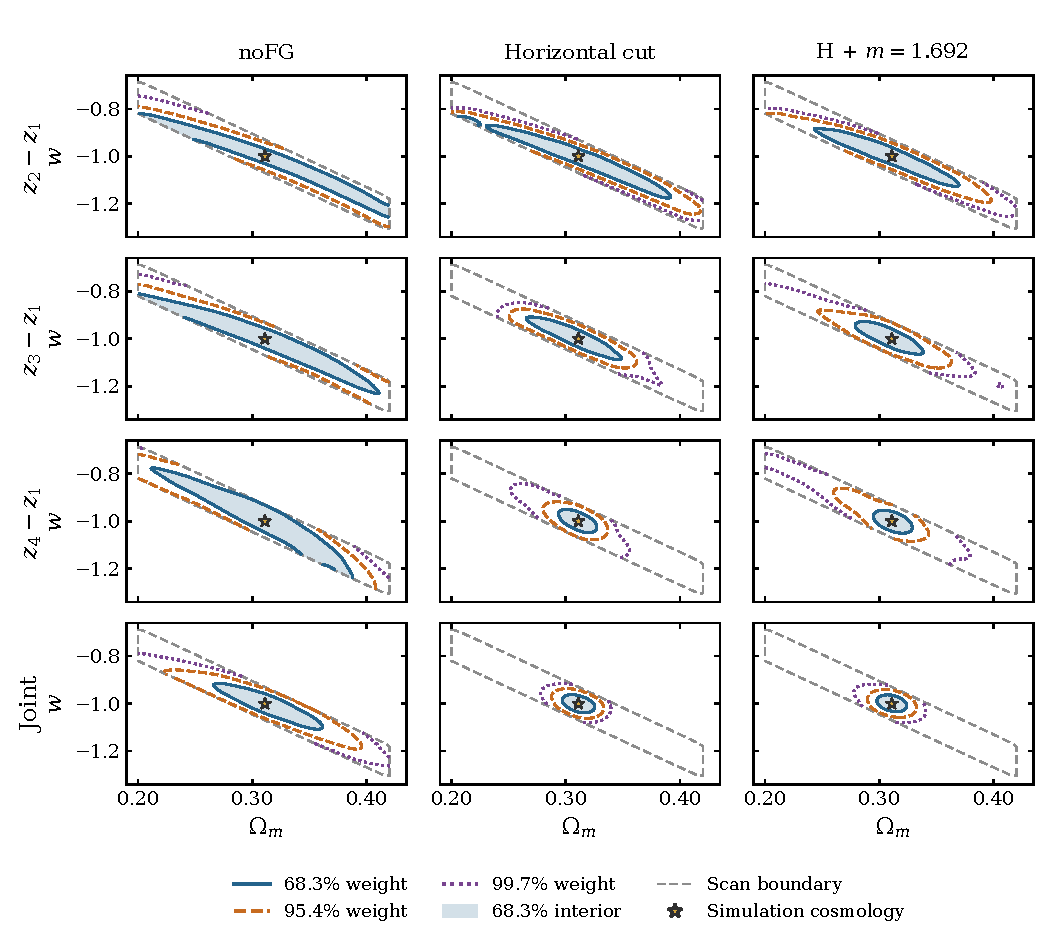
\includegraphics[width=\textwidth]{figures/fig__intrinsic_subtracted_contours__four_cases.pdf}
\caption{Smoothed parameter regions for the three redshift differences and their joint statistic in three foreground treatments. The weak-wedge case is retained in Supplementary Fig.~S2. Blue solid, orange dashed and purple dotted lines enclose 68.3, 95.4 and 99.7 per cent of the normalized weight; the 68.3 per cent interior is shaded. Grey dashed lines mark the scan boundary, and stars mark the simulation cosmology. Every panel uses the same weight interpolation, smoothing kernel and normalization domain. Common axis ranges retain boundary-reaching regions.}\label{fig:fourcases}
\end{figure*}

\subsection{Dependence on the wedge slope}\label{sec:wedgeareas}
Fig.~\ref{fig:areas} shows the joint area ratio $\mathcal R_f(m)=A_f(\mathrm{H}+m)/A_f(\mathrm{H})$ for the adopted smoothed weights, where $f$ denotes the enclosed weight fraction. Over the displayed slopes, the ratios span 0.81--1.05, 0.82--1.08 and 0.85--1.09 for $f=0.683$, 0.954 and 0.997, respectively. The variation is non-monotonic, and the smallest sampled area occurs at $m\simeq1.517$ at all three levels. At 68.3 per cent this is a 19.3 per cent reduction relative to the horizontal cut. The trend panel displays $m\le1.605$; the additional $m=1.692$ case is retained in Supplementary Table~S1 and Fig.~\ref{fig:smoothedcontours}.

\begin{figure*}
\centering
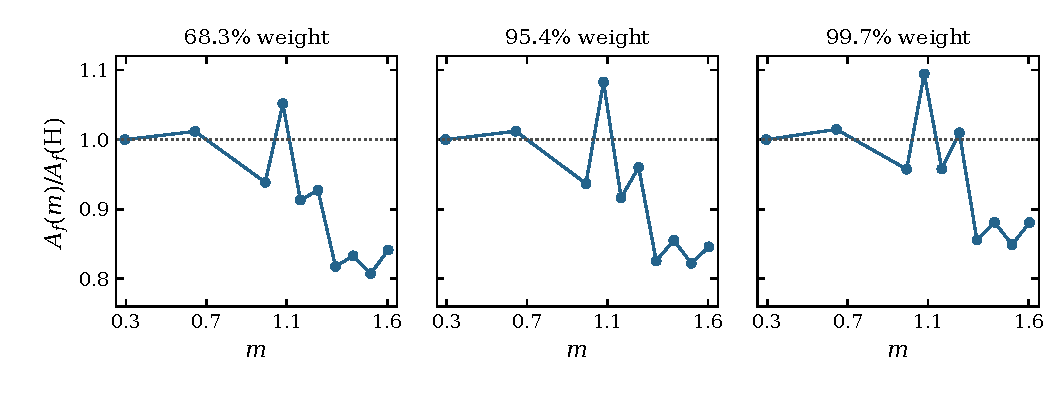
\includegraphics[width=\textwidth]{figures/fig__intrinsic_subtracted_contours__eleven_m_areas.pdf}
\caption{Joint-region areas relative to the horizontal cut for the adopted smoothed weight surface. Each panel gives one enclosed weight fraction; points are the ten sampled slopes up to $m=1.605$, and connecting lines guide the eye. Dotted lines mark unity. The trend display omits the endpoint $m=1.692$, whose result remains in Supplementary Table~S1 and Fig.~\ref{fig:smoothedcontours}.}\label{fig:areas}
\end{figure*}



Fig.~\ref{fig:smoothedcontours} compares three representative wedge cases with the horizontal-cut reference; Supplementary Fig.~S3 retains all eleven slopes. The weakest wedge almost coincides with that reference, while steeper wedges change both the area and the outer contour shape. The similar central contours and their modest area differences show that a larger removed Fourier region does not produce a monotonic change in these conditional constraints. Mode removal changes the measured genus response and its covariance weighting together; the comparison does not establish an optimal foreground cut for an observation.

\begin{figure*}
\centering
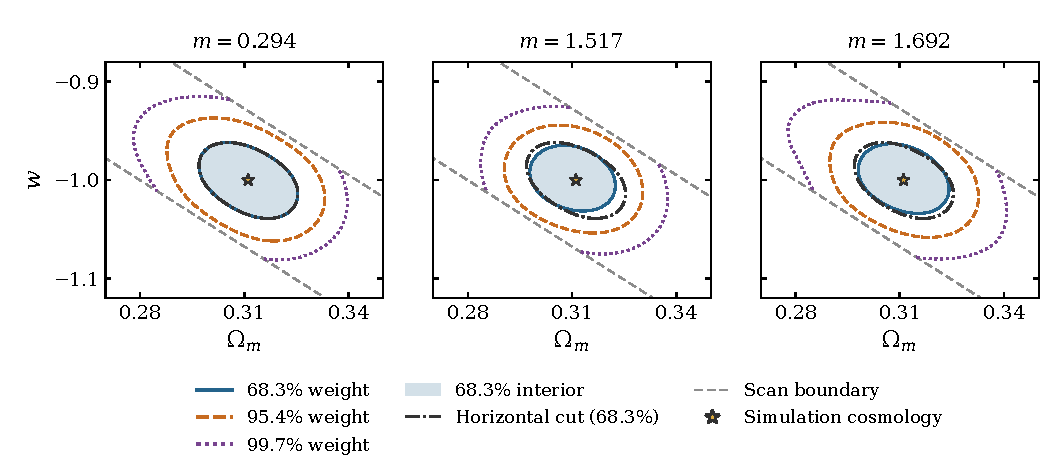
\includegraphics[width=\textwidth]{figures/fig__intrinsic_subtracted_contours__representative_smoothed.pdf}
\caption{Joint parameter regions for three representative wedge slopes, using the adopted smoothed weights. The full eleven-slope comparison is retained in Supplementary Fig.~S3. Blue solid, orange dashed and purple dotted lines enclose 68.3, 95.4 and 99.7 per cent of the weight within the common scan domain; blue shading marks the 68.3 per cent interior. The dark dash-dotted line is the horizontal-cut 68.3 per cent reference, processed with the same kernel. Grey dashed lines indicate the scan boundary, and gold stars indicate the simulation cosmology. All panels share the displayed ranges.}\label{fig:smoothedcontours}
\end{figure*}

\subsection{Numerical sensitivity of the parameter regions}\label{sec:numerics}
The parameter-area comparisons are sensitive to both field discretization and weight smoothing. In two pairs of almost identical trial cosmologies, separated by about $10^{-7}$ in their parameters, the horizontal-cut statistic jumps by 21.04 and 11.79 when an integer mesh count changes. Keeping $250^3$ cells removes these particular jumps (Table~\ref{tab:stability}). This test changes the cell size continuously with the AP-scaled box and is a diagnostic alternative to the main measurement, not an established converged estimator.

A separate 45-position line at fixed $w=-0.92451$ reveals another discontinuity even with fixed mesh counts: a discrete line-of-sight Fourier mode crosses the hard-cut boundary. The horizontal-cut statistic changes by $-23.37$ across a parameter separation of $10^{-7}$. Replacing the sharp cut by a hyperbolic-tangent transition suppresses this jump, but also changes the retained modes. Appendix~\ref{app:implementation} specifies the diagnostic filter. These examples identify two sources of numerical sensitivity; they do not establish that all residuals are numerical artifacts or that the alternative filter has converged.

\begin{table}
\centering
\caption{Changes in the horizontal-cut statistic across three close parameter pairs. The first two cross integer-mesh boundaries in the main scheme; the third crosses a hard-mask boundary in the fixed-mesh scheme. The same main covariance is used throughout.}\label{tab:stability}
\begin{tabular}{@{}lrrr@{}}\toprule
Pair & Main & Fixed mesh & Fixed + taper \\\midrule
Mesh boundary 1 & 21.037 & $-0.00181$ & $-0.000034$ \\
Mesh boundary 2 & 11.787 & $0.000015$ & $-0.00117$ \\
Mask boundary & $-0.000062$ & $-23.371$ & $-0.000021$ \\\bottomrule
\end{tabular}
\end{table}

For a matched 271-node subdomain, changing both the mesh prescription and filter changes the unsmoothed 68.3 per cent wedge-to-horizontal area ratio at $m=1.343$ from 0.497 to 1.184 with the original covariance, and to 1.220 when the tapered field has its covariance re-estimated. The regions at this level do not touch the subdomain boundary. This reversal tests robustness under different numerical and filtering choices; it does not isolate a pure discretization correction, and these subdomain values do not replace the full-scan results above.

Parameter-space smoothing produces a further change. At 68.3 per cent, it enlarges the noFG area by 2.49 and the horizontal-cut area by 6.71, changing their ratio from 10.28 to 3.81. Wedge areas increase by factors of 6.6--12.8. The smaller smoothed regions and the sampled minimum near $m=1.517$ therefore remain properties of the specified construction. They do not establish an optimal foreground cut or an improvement in observational precision.

\FloatBarrier % Keep result figures before the discussion and references.
\section{Discussion}\label{sec:discussion}
The first question concerns the evolution of the filtered genus. The measured curves change modestly across the four snapshots, while foreground removal changes their amplitudes and shapes substantially. Volume-fraction thresholds remove sensitivity to a uniform rescaling of density contrast, but do not remove evolution from changing morphology or tracer selection. The amplitude changes reported here are descriptive; their cross-redshift significance has not been calibrated.

The second question concerns the response to geometry. The tested incorrect mappings leave residuals after subtraction of the simulation-cosmology template, including in foreground-cut fields. This supports further investigation of redshift-dependent topology, but the numerical tests show that a response of the pipeline is not automatically a stable physical constraint. The simulation-cosmology zero is imposed by construction, and neither the template nor the regularized covariance has been validated with independent realizations. Internal resampling also omits modes larger than the available volume \citep{LacasaKunz2017InternalSSC}.

The third question concerns the meaning of the parameter areas. Mesh and mask discontinuities, empirical smoothing and finite-domain normalization materially affect them. Spatial convergence and independent statistical calibration are needed before interpreting them as parameter precision \citep{Kim2014GenusSystematics,Appleby2017,ApplebyBOSS2022}. The idealized cuts probe mode-loss geometries rather than an instrument-specific foreground model; realistic observations additionally require signal-loss calibration and survey selection modelling \citep{Cunnington2020ForegroundPNG,Cunnington2023ForegroundTransfer}. The present study identifies both a measurable geometric response and the numerical tests needed to develop it into a quantitative probe.

\section{Conclusions}\label{sec:conclusion}
We have examined how idealized foreground cuts affect the H\,I-weighted genus and its redshift-dependent response to AP mappings. Four Jiutian 1G snapshots at $0.10\le z\le0.59$ provide H\,I-weighted fields smoothed at $20\,h^{-1}\mathrm{Mpc}$. We compare their genus curves, subtract an intrinsic-evolution template and examine horizontal and wedge cuts across eleven slopes.

Foreground removal changes the topology substantially: the horizontal cut increases the fitted genus amplitude by about 4.6 while suppressing the density variance. Evolution across the sampled redshifts is modest, but endpoint changes alone omit intermediate variation. Incorrect mappings leave redshift-dependent residuals after template subtraction. Parameter-region areas, however, change under mesh and mask choices and parameter-space smoothing, so the current area ratios and sampled wedge minimum are not robust measures of cosmological precision.

These results motivate H\,I topology as a complement to conventional clustering statistics in the presence of foreground mode loss. Applying this approach to the SKA and related surveys will require realistic mock observations and a stable measurement definition \citep{Wang2015HITopologySKA}; no survey precision forecast is inferred here.

The present cuts omit instrumental response and residual foreground contamination. The intrinsic template depends on the simulation and H\,I population model, and the single-simulation covariance lacks independent calibration. The existing numerical comparisons expose sensitivity but do not demonstrate convergence or select a replacement estimator. Future work should establish numerical stability, propagate template uncertainty and test realistic foreground and survey treatments before quantitative cosmological inference.

\section*{Acknowledgements}
This work was supported by the National Natural Science Foundation of China (grant No. 12373005). We also wish to acknowledge the Beijing Super Cloud Center (BSCC) and Beijing Beilong Super Cloud Computing Co., Ltd (\url{http://www.blsc.cn/}) for providing HPC resources that have significantly contributed to the research results presented in this paper.

\section*{Data availability}
\todo{Confirm access conditions for the simulation catalogue and the repository or contact route for derived data and analysis code.}


\bibliographystyle{mnras}
\bibliography{references}

\appendix
\section{Smoothed weights and area calculation}\label{app:area}
We interpolate the weights $\exp(-\chi^2_{\rm int}/2)$ on a fixed triangulation of the 1285 sampled points, using the same geometry for every foreground treatment and redshift combination. The surface is evaluated on an $800\times800$ grid spanning $0.195\le\Omega_m\le0.425$ and $-1.325\le w\le-0.670$. Before Gaussian smoothing, missing weights outside the sampled convex hull are continued from the nearest sampled point, and the rectangular edges use a reflected continuation. These choices can affect the smoothed weights inside the hull and are part of the prescription.

We use the same Gaussian widths in parameter units for every surface, $\sigma_{\Omega_m}=0.0068836$ and $\sigma_w=0.0196033$. They originate from an empirical bandwidth based on 2.5 times the median nearest-neighbour distance in the unit-scaled scan rectangle, rather than from the covariance or an independent error calibration. This smoothing acts on the parameter weights, not on the measured genus curves or on the density field smoothed at $R=20\,h^{-1}\mathrm{Mpc}$.

Within the convex hull, weights are ordered from highest to lowest and the threshold is set where their cumulative sum reaches the chosen fraction of the total. The enclosed area is the number of selected grid elements times their area in $(\Omega_m,w)$. Thresholds are determined separately for each smoothed surface. For the joint surfaces, doubling the grid resolution at fixed parameter-unit kernel widths changes the areas by less than 0.6 per cent; this tests integration sampling, not the kernel choice or spatial convergence of the density field.

\section{Measurement details and diagnostic variants}\label{app:implementation}
At open boundaries, CIC weights are renormalized over cells inside the box to conserve deposited mass. The density contrast is zero-extended before Fourier transformation. For the Euler count, the cell-centred samples serve as vertices; an edge, face or cube is included only when all its vertices lie strictly above threshold. Each element is counted once, without identifying opposite faces.

The fixed-mesh diagnostic uses $250^3$ cells with $\Delta_i=L_i/250$, the same selected objects, $R=20\,h^{-1}\mathrm{Mpc}$ and 41 thresholds. The tapered variant multiplies the Fourier amplitude by
\begin{equation}
W=\tfrac12\left[1+\tanh\left(\frac{|k_\parallel|-k_{\rm cut}}{0.01\,h\,\mathrm{Mpc}^{-1}}\right)\right],
\end{equation}
where $k_{\rm cut}=0.1\,h\,\mathrm{Mpc}^{-1}$ for the horizontal cut and $\max(0.1\,h\,\mathrm{Mpc}^{-1},mk_\perp)$ for a wedge. Each variant uses its own simulation-cosmology intrinsic template. Comparisons first hold the main covariance fixed; the additional covariance test re-estimates it from the tapered simulation-cosmology fields with the same block method. Neither is an independent-realization calibration.

The 271-node area comparison uses identical nodes, triangulation and subdomain for both variants, with no parameter-space Gaussian smoothing. It evaluates highest-density regions from interpolated weights, re-determining the threshold for each surface. This diagnostic construction differs from the smoothed full-scan presentation; its area ratios are used only to assess sensitivity to the changes in measurement definition.

\section{Foreground-cut scales and wedge geometry}\label{app:kcut}
The minus sign in $\mathrm{d}\chi/\mathrm{d}\nu_{\rm obs}=-Y$ reverses the radial Fourier direction but leaves the symmetric cut in $|k_\parallel|$ unchanged. Equations~(\ref{eq:frequency_distance})--(\ref{eq:kcut_frequency}) follow by matching the phases $k_\parallel\Delta\chi$ and $2\pi\eta\Delta\nu_{\rm obs}$ in a locally narrow frequency interval. For $\chi_h=h\chi$, measured numerically in $h^{-1}\mathrm{Mpc}$, the corresponding conversion is $Y_h=hY$ and $k_{{\rm cut},h}=2\pi\eta_{\rm cut}/Y_h$.

An effective bandwidth $B_\nu$ gives a radial depth $L_\parallel\simeq YB_\nu$ and a fundamental scale $2\pi/L_\parallel$. This is not automatically the foreground threshold: removing a chosen number of fitted spectral components need not delete the same number of Fourier modes. The four coeval snapshots likewise do not specify an observing band or a light cone. At fixed numerical $k_{{\rm cut},h}$, the equivalent spectral period $2\pi/(Y_hk_{{\rm cut},h})$ varies with redshift.

With the adopted Fourier convention, the cut corresponds to a radial wavelength
\begin{equation}
\lambda_{\parallel,\rm cut}=\frac{2\pi}{k_{\rm cut}}
=62.83\,h^{-1}\mathrm{Mpc}.
\end{equation}
Thus $|k_\parallel|<k_{\rm cut}$ removes longer radial wavelengths, including the zero radial mode. It is not a cut on the total three-dimensional wavenumber. Since retained modes satisfy $k\geq |k_\parallel|\geq k_{\rm cut}$, their Gaussian amplitude transfer obeys $W_R(k)\leq\exp[-(k_{\rm cut}R)^2/2]=e^{-2}$ for $R=20\,h^{-1}\mathrm{Mpc}$. The corresponding power-transfer bound is $e^{-4}$; neither bound is a retained total-variance or information fraction.

For a transverse baseline of length $b$, a source at angle $\theta$ has geometric delay $|\tau|\leq b\sin\theta/c$. Using $k_\perp=2\pi b/(\lambda_{\rm obs}D_M)$ and $\lambda_{\rm obs}=c(1+z)/\nu_{21}$ gives
\begin{equation}
|k_\parallel|\leq m_{\rm geom}(z,\theta)k_\perp,\qquad
m_{\rm geom}=\frac{D_M(z)H(z)}{c(1+z)}\sin\theta.
\end{equation}
This is the geometric wedge relation \citep{SeoHirata2016Wedge}. The fixed slopes in our scans are controlled mask parameters, not redshift-dependent horizon boundaries at each snapshot.

The implemented retained-mode mask is
\begin{equation}
M(\boldsymbol k)=\boldsymbol 1_{|k_\parallel|\geq k_{\rm cut}}
\boldsymbol 1_{|k_\parallel|>mk_\perp}.
\end{equation}
The second factor is omitted for the horizontal-only case. The boundary is therefore the larger of $k_{\rm cut}$ and $mk_\perp$, with the stated equality conventions, rather than their sum. Their intersection is $k_\perp=k_{\rm cut}/m$. This also explains why a weak wedge can add little removal after smoothing.

\section{Block resampling and error propagation}\label{app:jackknife}
The $4\times4\times4$ partition uses the same normalized spatial labels across redshifts. Each open-complex vertex, edge, face or cube is assigned once to the block containing its lowest-index vertex. With $G_{ib}$ denoting its signed contribution to the negative Euler count, $t_{ib}=G_{ib}/V_i$ and $\sum_b t_{ib}=g_i$. The fraction $f_{ib}$ is the number of grid samples in the block divided by the total number. Equation~(\ref{eq:jk_loo}) removes that block's additive contribution and normalizes by the remaining grid volume. Cross-block elements are assigned by their anchor; they are not redefined as the topology of a freshly cut domain. No field reconstruction, filtering or threshold estimation is repeated for a leave-one-out replicate.

For a curve bin or any other scalar statistic $x$, the reported error is
\begin{equation}
\sigma_x=\left[\frac{B-1}{B}\sum_b(x^{(-b)}-\bar x)^2\right]^{1/2}.
\end{equation}
For redshift differences we subtract the same block-labelled replicates before taking their scatter. Their covariance therefore includes the cross terms:
\begin{equation}
C(g_i-g_1)=C_{ii}+C_{11}-C_{i1}-C_{1i}.
\end{equation}
The independent-error sum $C_{ii}+C_{11}$ is not used. The intrinsic template is held fixed when forming the covariance; its joint uncertainty with the measured evolution is not propagated.

For the equal-weight amplitude fit, define $u_j=(1-\nu_{f,j}^2)\exp(-\nu_{f,j}^2/2)$ and $a_j=u_j/\sum_k u_k^2$. Then $A=\boldsymbol a^{\mathsf T}\boldsymbol g$. Refitting the fixed template to each replicate is equivalent to $\sigma_A^2=\boldsymbol a^{\mathsf T}C_g^{\rm JK}\boldsymbol a$, and $\sigma_{AR^3}=R^3\sigma_A$. The percentages in Table~\ref{tab:amplitudes} are descriptive changes without assigned errors; uncertainties on a ratio $A_i/A_1$ would additionally require its paired cross-redshift propagation.

At the simulation cosmology the $250^3$ mesh cannot be divided into four equal integer lengths per axis: blocks have 62 or 63 grid samples along each direction. Using their actual fractions in Eq.~(\ref{eq:jk_loo}) does not by itself make Eq.~(\ref{eq:jk_cov}) an exact unequal-block jackknife prescription. The equal-block prefactor is a retained approximation. Alternative weighting, block size and independent-realization tests are needed to establish its statistical accuracy. OAS regularizes the inverse covariance and preserves the diagonal after rescaling; it does not supply that calibration or convert fixed-field resampling into uncertainty for the complete observational pipeline.
\label{lastpage}
\FloatBarrier
\end{document}
